\documentclass[a4paper]{article}
\usepackage{graphicx}
\usepackage[utf8]{inputenc}
\usepackage[english, serbian]{babel}

\title{MATF Elektronski časopis}
\date{2018}
\author{Dimitrije Špadijer, Božidar Antić, Nadežda Bogdanović}


\begin{document}
\maketitle
\newpage
\tableofcontents
\newpage

\section{Cilj projekta}

Razviti veb platformu koja će omogućiti sve neophodne funkcionalnosti za uređivanje elektronskog časopisa. Časopis izlazi dva puta godišnje i tematski je organizovan. Jezik časopisa je engleski.

\section{ Analiza sistema}

\subsection{Učesnici}

    Atributi: id, ime, prezime, korisničko ime, šifra, institucija, email, telefon(opciono), poštanski broj(opciono)
    Korisnici sistema imaju mogućnost upravljanja sopstvenim nalogom (promena korisničkog imena i šifre). Korisnici se međusobno razlikuju po ulogama i privilegijama koje su im dodeljene: Administrator, glavni urednik, urednik, recenzent, autor

    \subsubsection{Administrator}
    Administrator je korisnik sistema koji upravlja podešavanjima sistema: dodele korisničkih imena i šifara, dodavanje i uklanjanje novih korisnika, upravljanje nalozima, održavanje sistema - dakle stvari tehnološke prirode. On se odmah od početka korišćenja sistema nalazi u bazi podataka - ne registruje se. Iako su mu vidljivi svi podaci o svim korisnicima, radovima i brojevima časopisa, nema pravo dodele uloga (urednika i recenzenata), osim u slučaju dodele uloge glavnom uredniku.

    \subsubsection{Glavni urednik}
    Na vrhu piramide odlučivanja. Ne registruje se u sistem, administrator ga dodaje. Prilikom prijavljivanja prikazuje mu se u prvom delu prozora spisak novo-prijavljanih radova u sistemu označenih na upadljiv način. U drugom delu rada nalazi se paleta za pretraživanje: po autoru, imenu rada, datumu, statusu rada, statusu urednika, statusu autora.. Odabirom autora prikazuju mu se informacije o autoru. Odabirom rada prelazi se na radni prostor u kojem se ispisuje: naziv rada i informacije o autorima (ime, prezime, status svakoga od njih). Sam rad se nalazi u prilogu. G.urednik ima opciju da: rad odbaci bez konsutovanja sa ostalima i da rad prosledi uredniku. Iz padajuće liste bira urednika kojem šalje rad, u suprotnom, rad se arhivira kao odbačen. Glavni urednik ima pravo i da dodeli recenzente, urednike i da odluči koji će se rad objavljivati u kojem broju, da doda autora na crnu listu. Ima pristup odeljku "Upravljanje korisnicima" u kojem može da dodeli uloge urednicima/recenzentima, ili da ih oduzme. Ako želi da obriše nekog korisnika iz sistema, mora da pošalje poruku administratoru sistema. Takođe ima mogućnost ostavljanja komentar na rad. On odlučuje koji će se radovi naći u kojem broju.

    \subsubsection{Urednici}
    Urednici su specijalizovani za određene oblasti (oblast se pridodaje kao atribut). Primaju od g.urednika rad, čitaju ga i šalju predloge recenzentima. Urednik ima pravo da odbaci/prihvati rad, iako recenzenti misle da je rad za objavljivanje, ali onda treba da napiše obrazloženje. Ako urednik misli da je radu potrebna neka izmena, ima opciju da rad označi za menjanje, označava ga i otvara mu se polje gde unosi komentar urednika, koji objašnjava šta je sve potrebno promeniti. Ako komentar  na rad već postoji, on se učita u prostor za pisanje komentara i urednik ga menja ili briše i dodaje novi. Komentar urednika je opciona stavka. Po istom principu funkcionište i odbijanje/prihvatanje bez recenzije. Urednik prilikom logovanja na sistem ima u gornjem delu prozora spisak novih radova koje mu je poslao g.urednik. U donjem delu prozora je paleta za pretraživanje, opisana kao kod g.urednika. Odabirom na novi rad urednik ga ili odbaci, ili mu dodeli recenzente.

    \subsubsection{Recenzenti}
    Prilikom logovanja imaju spisak novih radova poslatih od urednika. Rad mogu da odbiju, i dalje nemaju više nikakva zaduženja vezana za taj rad. Takođe, mogu da pristupe i spisku svih dosadašnjih radova: prihvaćenih i odbijenih. Nakon pročitanog rada, recenzent popunjava formular za recenziju i objavljuje je. Potencijalni recenzent je onaj koji: je već recenzirao neki rad, ko je  kao korisnk čekirao polje "nemam ništa protiv da me kontaktirate za recenziranje nekog rada"

    \subsubsection{Autori}
    Dodatni atributi: broj dosadašnjih prilaganja radova, broj dosada objavljenih radova. Postoji i crna lista nepoželjnih autora koja sadrži ime autora i razlog zbog kog se nalazi na listi:  plagiranje, različiti vidovi varanja utvrđeni od strane ostalih korisnika sistema. Autori prijavljuju rad. Prilikom prijave ispunjavaju formular i označavaju da li je to novi rad, ili nova verzija rada koji je označen za ispravku. Ako u nekom trenutku žele da povuku rad, šalju zahtev za povlačenje rada.

\subsection{Časopis}
Atributi: ISSN, godina, naslov, g.urednik, urednici, minimalan i maksimalan broj radova po izdanju

\subsection{Rad}
    Atributi: broj, naslov, godina, imena autora, datum prve prijave, datum poslednje prijave, log prijava, rad u pdf formatu, recenzenti, urednik, status, broj verzija, objavljen

    Statusi rada:
    \begin{itemize}
        \item prijavljen: dobija status kada ga autor prijavi
        \item na recenziji: kada ga primi recenzent na recenziju
        \item na doradi: ovaj status dobija kada ga g.urednik/urednik označi da treba da ide na doradu
        \item povučen: ako je autor podneo zahtev za povlačenje rada
        \item odbijen bez recenzije: od strane g.urednika/urednika. U tom slučaju je potrebno priložiti komentar (funkcioniše isto kao kada se rad označava za doradu). Rad je odbijen bez recenzije i ako urednik nije mogao da pronađe recenzente koji žele da recenziraju rad, a sam nije želeo da čita ceo rad
        \item odbijen sa recenzijom
        \item prihvaćen bez recenzije: slično kao odbijen bez recenzije, potrebno je ostaviti komentar
        \item prihvaćen sa recenzijom
    \end{itemize}


\subsection{Prijavljivanje i registrovanje korisnika}
Prilikom registrovanja, korisnik ima mogućnost da označi opciju "nemam ništa protiv ako želite da me odaberete kao recenzenta". Ako ovu opciju nije čekirao, može to da učini kasnije kada se prijavi.
\begin{itemize}
    \item Registrovanje: popuni se formular i pošalju podaci. Administrator ih prima i šalje šablon1 u kojem korisnika obaveštava koje mu je korisničko ime i šifra
    \item Prijavljivanje: korisnik popuni formular i time se uloguje
\end{itemize}

\subsection{Komunikacija među korisnicima}
Korisnik odabere šablon, otvori mu se radna površina za pisanje u koju se šablon učita. On taj šablon može sačuvati i ima opciju da ga pošalje, čime se šablon automatski šalje na mejl drugog saučesnika u komunikacji. Korisnik može i napraviti novi šablon i obrisati ga, ako nije predefinisan od strane sistema, kao što su dole navedeni šabloni.
\begin{itemize}
\item Administrator ostalim korisnicima: šabloni 1 (uspešno registrovanje) i 2 (uspešna/neuspešna promena ličnih podataka)
\item G.urednik urednicima: šablon 3 (o novopristiglom radu)
\item G.urednik administratoru: šablon 4 (o brisanju korisnika iz sistema)
\item Urednik recezentima: šablon 5 (predlog rada za recenziranje)
\item Urednik autoru: šablon 6 (o tome kako je rad prihvaćen i šta treba da priloži) i  šablon 7 (odbijen i obrazloženje)
\item Recenzent uredniku: šablon 7 (o tome da li odbija ili prihvata recenziju)
\end{itemize}

\subsection{Životni ciklus rada}
\subsubsection{Prijavljivanje}
Rad prijavljuje autor koji je ujedno i odgovorno lice za taj rad. Spisak autora koje rad sadrži kao atribut mogu biti reference na autore već poznate sistemu, inače o autoru će biti napravljen zapis u sistemu koji će biti moguće koristiti kao njegov kontakt u slučaju da je to potrebno (npr. poziv za učlanjenje).
\subsubsection{Dodeljivanje urednicima i recenzentima}
Rad je inicijalno prikazan glavnom uredniku koji ga dodeljuje uredniku. On zatim "nudi" rad recenzentima koji imaju mogućnost da prihvate ili odbiju tu ulogu. Obaveštenja o dodelama radova i ponudama recenzentskih uloga su realizovana putem slanja šablona (opisanim u delu 6) i praćena su akcijama sistema.
\subsubsection{Recenziranje}
Recenzent može prihvatiti rad koji mu je ponuđen na recenziju od strane urednika nakon čega automatski biva dodeljen tom radu. Od njega se očekuje da popuni formular koje će sadržati delove koji su upućeni autoru/autorima i uredniku. Nakon popunjavanja objavljuje svoju recenziju koja će biti vidljiva uredniku, koji preuzima dalje akcije.
\subsubsection{Komentarisanje rada od strane urednika}
Rad može biti komentarisan od strane glavnog urednika i urednika i to u slučajevima kada je rad odbijen sa komentarom, koji će autor moći da pročita kao objašnjenje za preduzetu akciju, ili kada se rad označava za doradu, čime se autoru stavlja do znanja koje su to promene koje se zahtevaju.
\subsubsection{Ažuriranje}
Nakon što je rad od strane urednika označen za doradu, autor ima mogućnost da izmenjenu verziju rada ponovo prijavi. U tom slučaju potrebna je ponoviti i dodelu recenzenata. Kao u slučaju prvobitne dodele, uredniku je ponuđen spisak recenzenata na kome bi favorizovani bili oni koji su na tom radu već imali recenzentsku ulogu.
\subsubsection{Menjanje statusa}
Status rada je inicijalno postavljen na "prijavljen" i može biti promenjen akcijama korisnika sistema. Moguća stanja i akcije koje dovode do tih stanja su navedene u delu 2.3.
%\subsection{Prijavljivanje rada kao plagiran/uvredljiv sadržaj}
%Ovo pravo imaju samo registrovani korisnici.


\subsection{Sistemska podešavanja}
Obavlja ih administrator: upravljnje podacima u bazi, dodavanje novih korisnika i uklanjanje postojećih... Na nivou sistema treba da postoji log svih aktivnosti koji treba da bude vidljv administratoru i glavnom uredniku

\subsection{Šabloni i formulari}
Sadržaj šablona i formulara biće priložen nezavisno od ovog dokumenta u odeljku "Prilozi (Attachments)"

\section{Slučajevi upotrebe}

\subsection{Promena podešavanja časopisa}
\begin{itemize}
    \item Akter: Administrator sistema
    \item Kratak opis: Administrator menja podešavanja časopisa
    \item Osnovni tok događaja:(ponavljati korak 2 željeni broj puta)
        \begin{enumerate}
            \item Administrator pristupa obrascu za menjanje podataka
            \item Administrator unosi podatke u formu
            \item Adminstrator pokušava da sačuva nove podatke
            \item Novi podaci su sačuvani na sistemu
        \end{enumerate}
    \item Alternativni tok događaja:
        \begin{enumerate}
            \item Sistem ne može da sačuva nove podatke
                \begin{enumerate}
                    \item Administrator proverava da li su podaci validni u odnosu na već definisanu bazu podataka. Ponovo pokušava da sačuva podatke, ako ne uspe, prelazi na korak 1.b. alternativnog toka
                    \item Administrator proverava internet konekciju i uspešno je podešava. Ponovo pokušava da sačuva podatke, ako ne uspe, prelazi na korak 1.c alternativnog toka
                    \item Administrator proverava da li je funkcionalnost slanja podataka preko forme dobro implementirana. Ako nije, popravlja to i pokušava ponovo da sačuva podatke. Ako ne uspe, prelazi na korak 1.d alternativnog toka
                    \item Ozbiljna greška sistema. Administrator traži grešku i pokušava da je otkloni.
                \end{enumerate}
        \end{enumerate}
\end{itemize}

\begin{figure}[hbt!]
    \centering
    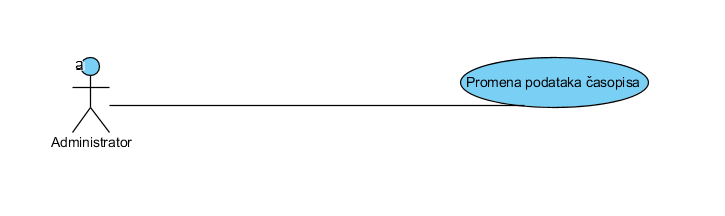
\includegraphics[width=\linewidth]{USeCasePromenaPodatakaCasopisa.png}
    \caption{UseCase Promena podataka časopisa}
    \label{fig:my_label}
\end{figure}

\subsection{Prijavljivanje korisnika}
\begin{itemize}
    \item Akter: Korisnik sistema (Administrator, Glavni urednik, Urednik, Recenzent, Autor)
    \item Kratak opis: Korisnik unosi potrebne podatke kako bi se ulogovao u sistem
    \item Osnovni tok događaja:
        \begin{enumerate}
            \item Korisnik unosi svoju email adresu i sifru u polja koja su za to predoredjena
            \item Pokusava da se prijavi na sistem
            \item Nakon uspesnoj autentikaciji korisnika prikazuje mu početna stranica u zavisnosti od uloge:
            \begin{enumerate}
                \item Administrator - admin panel za upravljanje sistemom
                \item Glavni urednik - lista novopristiglih radova
                \item Urednik - lista radova koji su poslednji dodeljeni od strane glavnog urednika
                \item Recenzent - lista radova koji su poslednji ponudjeni za recenziju od strane urednika
                \item Autor - listu svojih radova
            \end{enumerate}
        \end{enumerate}
    \item Alternativni tok događaja:
        \begin{enumerate}
            \item Autentikacija korisnika nije uspela
                \begin{enumerate}
                    \item Nakon 2. koraka sistem ispisuje poruku o neuspešnoj autentikaciji.
                    \item Korisnik ponavlja korake 1. i 2.
                \end{enumerate}
        \end{enumerate}
\end{itemize}

\begin{figure}[hbt!]
    \centering
    \includegraphics[width=0.8\linewidth]{UseCasePrijavljivanjeKorisnika.png}
    \caption{UseCase Prijavljivanje korisnika}
    \label{fig:my_label}
\end{figure}

\subsection{Registracija korisnika}
\begin{itemize}
    \item Akter: Korisnik sistema (budući) (Glavni urednik, Urednik, Recenzent, Autor)
    \item Kratak opis: Korisnik unosi potrebne podatke kako bi se registrovao u sistemu
    \item Osnovni tok događaja:
        \begin{enumerate}
            \item Korisnik unosi podatke u formular koji mu se prikazuje nakon zahteva za registracijom (dok ne uradimo screenshot forme, ovo je placeholder formular sadrzi polja: First Name, Last Name, Title, Email, Confirm email, Password, Repeat Password, URL, Phone, Country, (check option) Available for reviewing role, Google ReCaptcha)
            \item Korisnik pokušava da se registruje
            \item Korisniku se prikazuje naredna stranica na kojoj se od njega zahteva da ulaskom na link koji mu je poslat na email, potvrdi svoj email
            \item Nakon potvrde svoje email adrese korisnik je uspešno registrovan (i ima Autorsku ulogu)
        \end{enumerate}
    \item Alternativni tok događaja:
        \begin{enumerate}
            \item Neko od obaveznih polja nije popunjeno
                \begin{enumerate}
                    \item Nakon 2. koraka sistem ispisuje poruku o grešci i zahteva od korisnika da unese podatke koji fale u obaveznim poljima i ta polja bivaju označena.
                    \item Korisnik popunjava tražena polja.
                    \item Korisnik zatim ponavlja korak 2 iz glavnog toka.
                \end{enumerate}
            \item Vrednosti u poljiva Confirm email i Repeat Password ne odgovaraju vrednostima u poljima Email i Password
                \begin{enumerate}
                    \item Nakon 2. koraka sistem ispisuje poruku o grešci i obaveštava korisnika o nepoklapanju podataka u datim poljima.
                    \item Korisnik ponovo popunjava sporna polja.
                    \item Korisnik zatim ponavlja korak 2 iz glavnog toka.
                \end{enumerate}
            \item Neko od polja ne odgovara formatu koji je za to polje zadat regularnim izrazom
                \begin{enumerate}
                    \item Nakon 2. koraka sistem ispisuje poruku o grešci i zahteva od korisnika da unese podatke u odgovarajućem formatu za polja koja označava na neki način.
                    \item Korisnik ponovo popunjava tražena polja.
                    \item Korisnik zatim ponavlja korak 2 iz glavnog toka.
                \end{enumerate}
            \item ReCaptcha ne prepoznaje korisnika kao živu osobu
                \begin{enumerate}
                    \item Nakon 1. koraka sistem ne dozvoljava korisniku da nastavi sa registracijom.
                    \item ReCaptcha se reinicijalizuje.
                    \item Korisnik ponovo pokušava da "reši"\ ReCaptcha.
                    \item Korisnik ponavlja korak c) ovog alternativnog toka 4 dok ne bude moguće preći na korak 2 glavnog toka.
                    \item Prelazi na korak 2 glavnog toka.
                \end{enumerate}
        \end{enumerate}
\end{itemize}

\subsection{Promena ličnih podataka}
\begin{itemize}
    \item Akter: Korisnik sistema (Administrator, Glavni urednik, Urednik, Recenzent, Autor)
    \item Kratak opis: Korisnik želi da promeni neke od ličnih podataka
    \item Osnovni tok događaja:
        \begin{enumerate}
            \item Korisniku se prikazuje forma slična onoj koja je korišćena za registraciju, bez pojedinih polja ReCaptcha na kojoj korisnik menja željene podatke.
            \item Korisnik pokušava da promeni podatke.
            \item Novi podaci korisnika su sačuvani.
            \item Nakon uspešne promene podataka sistem obaveštava korisnika o uspešnoj akciji.
        \end{enumerate}
    \item Alternativni tok događaja:
        \begin{enumerate}
            \item Medju promenjenim podacima je i email adresa
                \begin{enumerate}
                    \item Nakon 2. koraka sistem ispisuje poruku uspešnosti promene svih korisničkih podataka osim email adrese. Ispisuje se obaveštenje da korisnik treba da potvrdi svoju novu email adresu tako što će posetiti link koji mu je na tu adresu poslat.
                    \item Korisnik prelazi na korak 3 glavnog toka podataka.
                \end{enumerate}
            \item Neko od obaveznih polja nije popunjeno ili neko od polja ne odgovara formatu koji je za to polje zadat regularnim izrazom
                \begin{enumerate}
                    \item Nakon 2. koraka sistem ispisuje poruku o grešci i obaveštava korisnika da podaci nisu uspešno izmenjeni.
                    \item Korisnik se vraća na korak 1 glavnog toka.
                \end{enumerate}
        \end{enumerate}
\end{itemize}

\subsection{Promena korisničkih podataka}
\begin{itemize}
    \item Akter: Administrator
    \item Kratak opis: Korisnik želi da promeni neke od ličnih podataka drugih korinika
    \item Osnovni tok događaja:
        \begin{enumerate}
            \item Administratoru se prikazuje panel u kojem se nalazi spisak korisnika kojima može menjati lične informacije.
            \item Administrator bira željenog korisnika.
            \item Administratoru se prikazuje formular na kome može menjati lične podatke korisnika (sve osim email-a).
            \item Nakon uspešne promene podataka sistem obaveštava administratora o uspešnoj akciji.
        \end{enumerate}
    \item Alternativni tok događaja:
        \begin{enumerate}
            \item Neko od obaveznih polja nije popunjeno ili neko od polja ne odgovara formatu koji je za to polje zadat regularnim izrazom
                \begin{enumerate}
                    \item Nakon 2. koraka sistem ispisuje poruku o grešci i obaveštava administratora da podaci nisu uspešno izmenjeni.
                    \item Administrator se vraća na korak 3 glavnog toka.
                \end{enumerate}
        \end{enumerate}
\end{itemize}

\subsection{Odabir prihvaćenih radova za tekuće izdanje časopisa}
\begin{itemize}
    \item Akter: Glavni urednik časopisa
    \item Kratak opis: Glavni urednik časopisa razmatra sve radove koji su prihvaćeni i vrši odabir radova koji će ući u tekuće izdanje časopisa.
    \item Osnovni tok događaja:(Ponavljati korake 3, 4, 5. i 6. dok se postigne traženi broj radova ili traženi broj stranica za tekuće izdanje)
        \begin{enumerate}
            \item Glavni urednik upućuje upit sistemu za sve prihvaćene radove koji nisu objavljeni ni u jednom dosadašnjem izdanju časopisa.
            \item Sistem vraća spisak svih takvih radova.
            \item Glavni urednik pregleda sledeći rad.
            \item Glavni urednik donosi odluku da li će rad ući u tekuće izdanje časopisa.
            \item Ukoliko će rad ući u tekuće izdanje: Glavni urednik šalje zahtev sistemu da se rad ubaci u radnu verziju tekućeg izdanja časopisa.
            \item Sistem dodaje rad u radnu verziju tekućeg izdanja.
        \end{enumerate}
    \item Alternativni tok događaja:
        \begin{enumerate}
            \item  (2) Sistem ne vraća uspešno spisak prohvaćenih radova. Glavni urednik pokušava ponovo da izvrši korak 1. Ukoliko ne uspe, obraća se administratoru časopisa.
            \item (3) Sistem ne vraća uspešno sledeći rad koji glavni urednik želi da pregleda. Glavni urednik pokušava ponovo da pregleda rad. Ukoliko ne uspe, obraća se administratoru časopisa.
            \item (6) Sistem ne dodaje rad u radnu verziju tekučeg izdanja. Glavni urednik pokušava ponovo. Ukoliko ne uspe, obraća se administratoru časopisa.
        \end{enumerate}
\end{itemize}

\begin{figure}[hbt!]
    \centering
    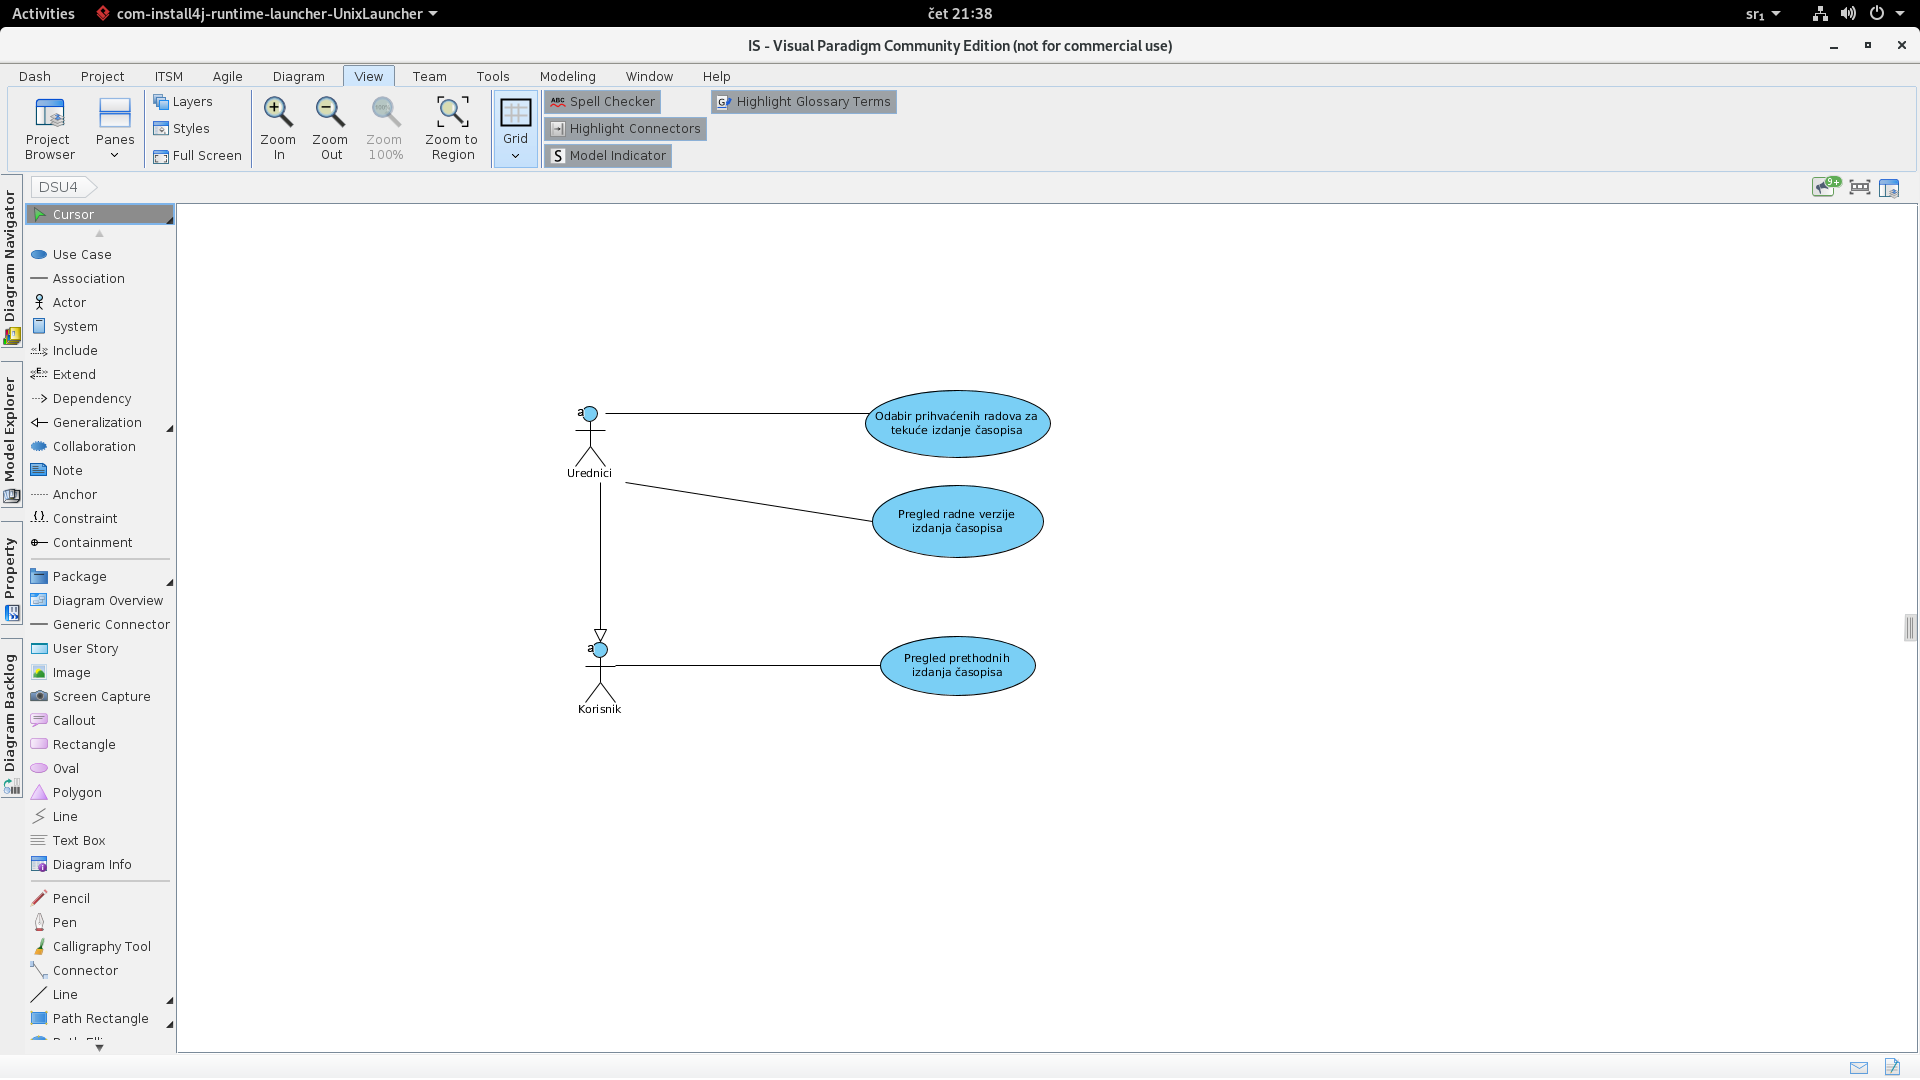
\includegraphics[width=\linewidth]{slucaj_upotrebe_urednici.png}
    \caption{Upravljanje časopisom}
    \label{fig:my_label}
\end{figure}


\end{document}
